\documentclass[a4paper,12pt]{article}
\usepackage{graphicx}
\usepackage{float}
\begin{document}

\title{Cubeviz User Manual}
\maketitle

\tableofcontents

\section{Introduction}

Cubeviz is a lightweight visulisation tool designed for use with Iris and Cartopy.
It allows you to quickly and easily load a file, and then view plots of the cubes
within it.

You are able to select which cube from the file you would like to plot, and,
for cubes with more than 2 dimensions, you are able to choose to plot any
2D slice of the cube.

Further, you have numerous options regarding how the cube will be plotted,
from the type of graph, to drawing coastlines, all of which are explained in
this manual.

\vspace{4mm}

This manual will help you get help you get started with Cubeviz, and guide you
through the features that it offers. For hints whilst using the
program, hold your mouse over the relevant section to produce a tool
tip describing its function.

\pagebreak

\section{Installation}

\pagebreak

\section{Getting Started}

\begin{figure}[h]
\centering
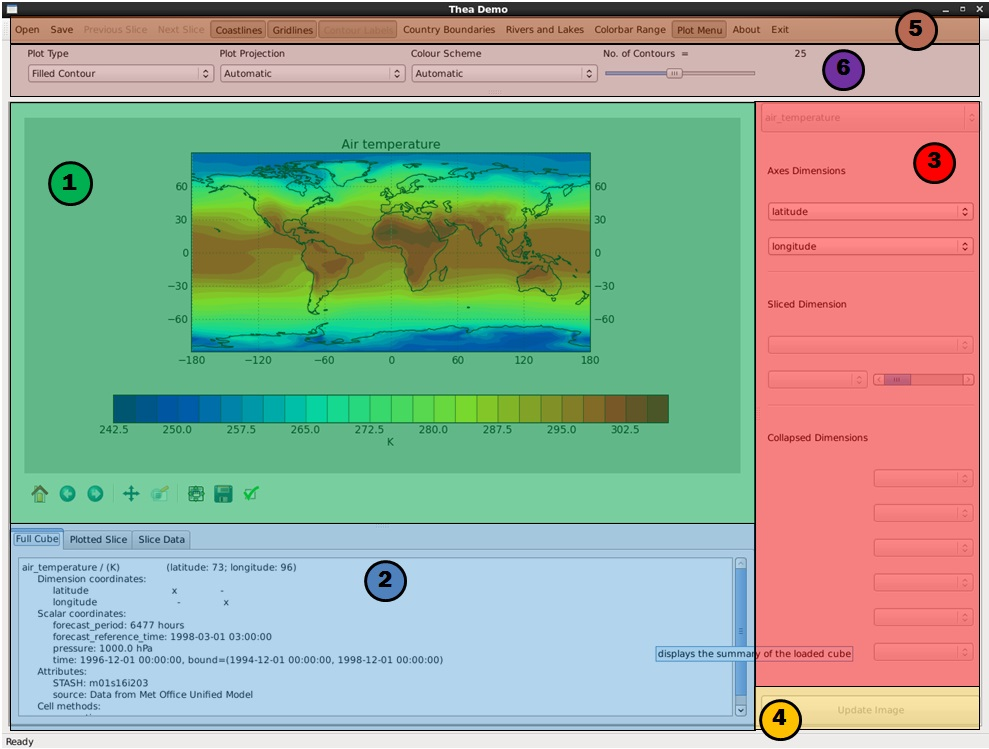
\includegraphics[width=130mm]{theaGuideJPEG.jpg}
\caption{This figure shows the main window of the application, broken down into
its key components.}
\label{overflow}
\end{figure}

The main window can be broken down into a few main segments;

\begin{enumerate}

\item
\emph{Embedded Matplotlib Display:} Where the plot is displayed.

\item
\emph{Cube Information:} Displays a summary of the cube and the slice, and
shows the data within the slice.

\item
\emph{Cube Menu:} Allows selection of which slice is plotted.

\item
\emph{Update Button:} Replots the cube.

\item
\emph{Toolbar:} Numerous Actions such as open and save.

\item
\emph{Plot Menu:} Allows selection of how the cube is plotted.


\end{enumerate}

\subsection{Embedded Matplotlib}

The plot is displayed in an embedded matplotlib window. This means that all of
the functionality that you would have using matplotlib from terminal will still
be present here.

For example, by clicking the magnifying glass icon in the matplotlib toolbar,
you are able to zoom in on any area of the plot by dragging a rectangle around
the section that you would like to enlarge. Equally, you are also able to
enlarge a region by specifying the range over which the  graph will be plotted.
This is done by clicking on the green tick, clicking ok, and then specifying
the max and min of the axes range.

You can also pan and zoom by clicking the pan button, can save using the save
button, and can adjust the position of the plot using the configure subplots
button.

If you mouse over the plot, you will discover that the current posistion of the
mouse will be displayed to the right of the toolbar.

\subsection{Cube Information}

This pannel contains all of the information about the cube. There are three tabs
to select from, Full Cube, Cube Slice, and Slice Data.

\begin{itemize}

\item
\emph{Full Cube:} This tab will show you the summary of the cube that is
currently loaded.

\item
\emph{Cube Slice:} This tab will display the summary of the slice of the cube
that is currently being plotted. (note that this will be the same as the full
cube if the cube has fewer than 3 dimensions).

\item
\emph{Slice Data:} This tab will display the raw data contained within the
current slice in the form of a table.

\end{itemize}

\subsection{Cube Menu}

The Cube Options sections is split into 4 parts.

\begin{itemize}

\item
\emph{Select Cube:} This drop down box allows you to select which cube you
would like to view from the list of cubes in the current file. If there is
only one cube in the file, this box will be disabled.

\item
\emph{Axes Dimensions:} These 2 drop down boxes contain the coordinates that
will be placed on the axes of the plot. For example, if the boxes contained
height and time, then the application will produce a plot of height against
time.

You are able to choose any of the dimensions from the drop down box.

The order of the two boxes is not important, (i.e. a selection of latitude
and longitude will produce the same result as longitude and latitude.

\item
\emph{Sliced Dimension:} This is the dimension in which the slices will
be taken. The next and previous slice buttons will move along slices in this
dimension, and setting the colorbar across all slices refers to this dimension.

The top box contains the dimension that is currently being sliced, while the
box below it contains the value apon which that dimension will be collapsed
for this slice.

You are able to select the desired dimension using the drop down box, and
can choose which slice along this dimension is taken by using either the
slider or the drop down box.

\item
\emph{Collapsed Dimensions:} The remaining dimensions are placed in this area.
The names of the remaining dimensions will apear alongside a drop down list.

To obtain a 2D cube which can be plotted, the program will collapse these
dimensions down onto the values specified in the boxes. You are able to select
which value to collapse onto by using the drop down boxes.

\item
\emph{N.B:} For cubes which contain anonymous dimensions, you will find that
the coordinate name will be set to *ANONYMOUS* (with a number atatched to
distinguish between multiple anonymous coordinates.)

The application will function as normal with these coordinates, however it
will fill the drop down boxes with the numbers 0 - (n-1) (where n is the size
of the dimension) instead of the values of the coordinate as these do not exist
for anonymous dimensions.

\end{itemize}

\subsection{Update Button}

This button will cause the plot to be redrawn. The changes that you make to
the plot will not be executed until the update button is pressed.

\subsection{Toolbar}

The main toolbar contains numerous options and actions:

\begin{itemize}

\item
\emph{Open:} Brings up a file browser from which you are able to select a to
file open

\item
\emph{Save:} Opens a window which allows you to save the current image in a
specified location with a specified name in a number of different file types
including jpeg and png

\item
\emph{Previous Slice:} Only enabled if the cube has three or more dimensions.
This will move you to the slice with a coordinate index of the sliced dimension
which is one lower than the current index.

\item
\emph{Next Slice:} Only enabled if the cube has three or more dimensions.
This will move you to the slice with a coordinate index of the sliced dimension
which is one higher than the current index.

\item
\emph{Source Code: } Clicking this button will open up a new window containing
code that is able to recreate the currently displayed image. 

\item
\emph{Coastlines:} Toggle the plotting of coastlines on and off. This will be
disabled if the plot is not detected to be a lat/lon plot.

\item
\emph{Gridlines:} Toggle whether gridlines should be drawn onto the plot.

\item
\emph{Contour Labels:} Toggle the labelling of the contours. Only enabled if
the plot type is Contour.

\item
\emph{Country Boundaries:} Toggle the marking of country borders.

Will only be enabled if the plot is detected to be lat/lon.

Note: This will also give a more detailed representation of the coastlines,
but will slow down the plotting of the graph.

\item
\emph{Rivers and Lakes:} Toggle the marking on of major lakes and rivers.

This will only be enabled if the plot is detected to be lat/lon.

\item
\emph{Colorbar Range:} Opens a window giving you options about how the colorbar
is set. See section 4 for more details.

\item
\emph{Plot Menu:} This will toggle the plot menu on and off. See section 3.6
for more details on the Plot Menu.

\item
\emph{About:} Gives brief general and copywrite information about the
application.

\item
\emph{Exit:} Closes the application.

\end{itemize}


\subsection{Plot Menu}

This menu contains options which affect the visual appearence of the plot.

The menu can be toggled on and off by clicking the plot menu button in the
toolbar.

\begin{itemize}

\item
\emph{Plot Type:} This option allows you to select the type of graph you would
like to plot. Choose from Contour, Filled Contour and pcolormesh (Block Plot).

\item
\emph{Plot Projection:} This option allows you to select the type of plot
projection that you would like.

\vspace{4mm}

\emph{N.B.} At the time of writing, some bugs in Cartopy make many of the
projections very tempremental. (This is known about and being fixed)

Some of the projections will return just a dot. If this is the case then you
should be able to zoom in on them (see section 3.1)

Others will plot data in areas outside of the earth or will have a discontinuity
part way across.

Some may even cause the application to stop working. In this case, exit the
application using, clicking 'force close' if required, and then restart the
program.

Which projections fail depends on the plot type being used and on the data
being plotted. If in doubt, leave the projection as automatic. 

\item
\emph{Color Scheme:} This option allows you to select a color scheme for the
plot. The colour schemes availiable are the brewer palletes that were compatible
with Iris at the time of writing. 

\item
\emph{No. of Contours:} This option allows you to select the number of contours
to plot.

This option will be disabled if the plot type is pcolormesh.

If the Color Scheme has fewer colors than the number of contours, then multiple
contours will be set to one color.

\end{itemize}

\pagebreak

\section{Colorbar Options Window}

In this window, you are able to change which values the colorbar will be set
between.  The current maximum and minimum of the range will be shown in the
max and min boxes.

\begin{figure}[h]
\centering
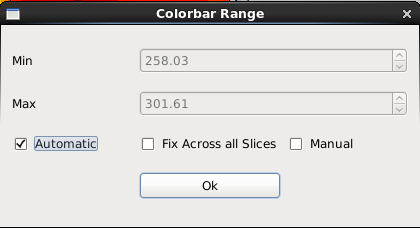
\includegraphics[width=80mm]{colorbarRangeDiagram.png}
\caption{This figure shows the main window of the application, broken down into
its key components.}
\label{overflow}
\end{figure}

\subsection{Automatic Selection}

By default, the application will scan through the values in the current slice,
and find the maximum and the minimum values. It will then set the lowest color
to the minimum value, and the highest color to the maximum value, and fill
in everything else.

\subsection{Fixed Colorbar}

If you are looking to compare different slices, it may be useful for the
colorbar to be constant, instead of changing itself from slice to slice. To
do this, it often makes sense to set the colorbar to the max and min of the
entire set of slices, instead of just the current slice, and that is exactly
what is done by this option.

For a good example of where this is useful, see the tutorial section 5.2.3.

\subsection{Manual Selection}

Alternatively, you might wish to set your own range. To do this, simply click
Manual Selection and then enter your chosen values into the boxes.

\pagebreak

\section{Tutorial}

In this short tutorial, I will step you through how to load your first cubes,
\vspace{4mm}and then introduce the options availiable to you in Cubeviz. \\
\vspace{4mm}The files used in this tutorial are from the Iris-Sample-Data. \\*
If you do not have these files already, then they can be found at

https://github.com/SciTools/iris-sample-data

\subsection{2D Cubes}

We will start with a simple 2D cube which holds data on gloabl air temperature.

\subsubsection{Load a File}

\begin{figure}[H]
\centering{}
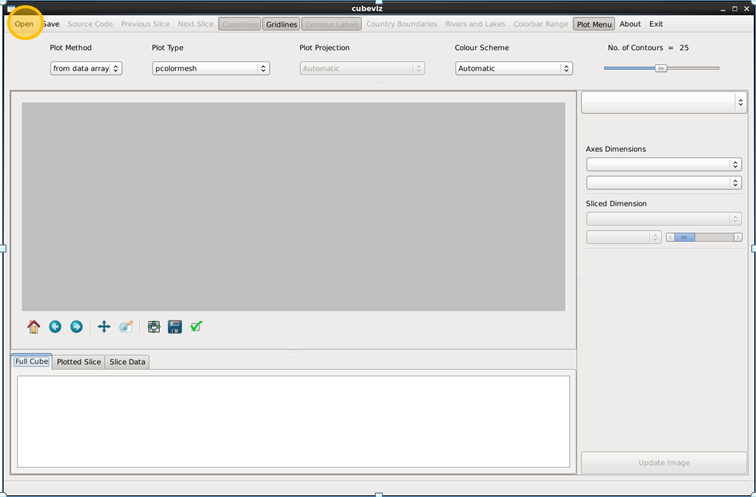
\includegraphics[width=90mm]{tute1.PNG}
\caption{Click here to open a new file.}
\label{overflow}
\end{figure}

To load this file, simply click on the 'Open' button found at the top left
of the screen. This will open a file browser. From here, navigate to your
version of the iris-sample-data folder, select the file named
'A1B.2098.pp' and click open.

\begin{figure}[H]
\centering{}
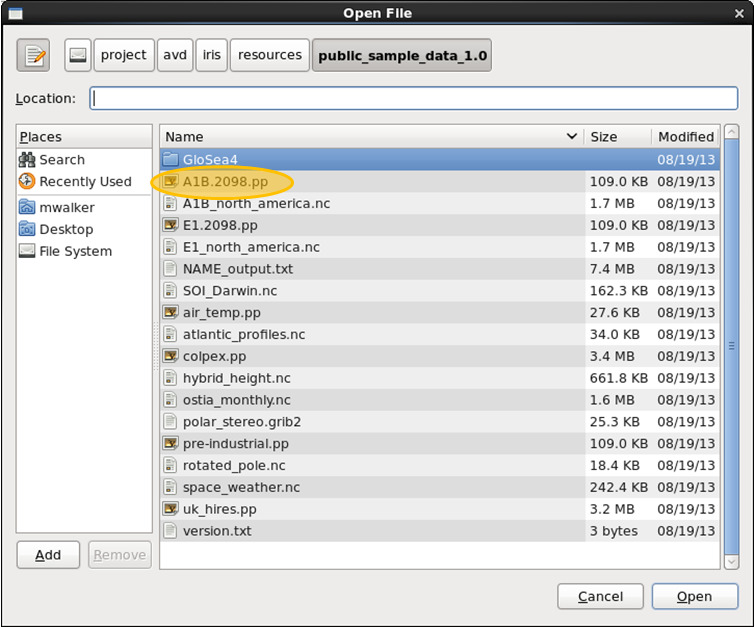
\includegraphics[width=90mm]{tute2.PNG}
\caption{Select the A1B.2098.pp cube}
\label{overflow}
\end{figure}

\subsubsection{Screen Layout}

The cube should now be loaded, and should have been plotted on the left of
your screen. To the right of the screen, you will see that
the axes dimension boxes and the select cube box have been filled, but not the
Sliced Dimension box. This is because the cube has only 2 dimensions.

\begin{figure}[H]
\centering
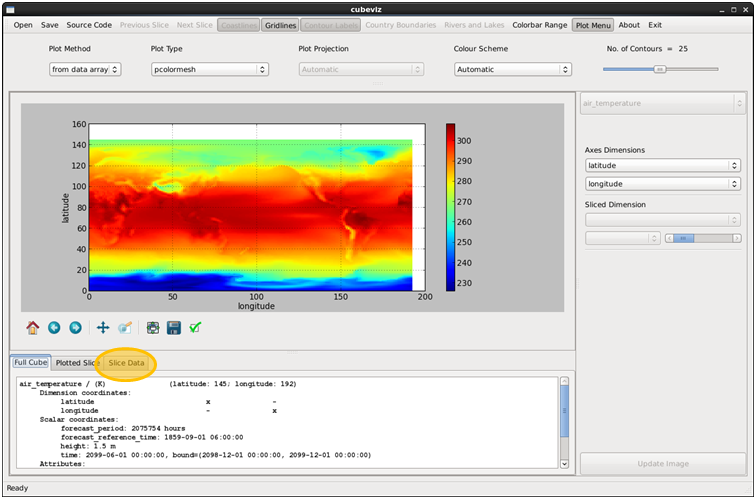
\includegraphics[width=90mm]{tute3.PNG}
\caption{Clear here to view the data in the cube.}
\label{overflow}
\end{figure}

If you look to the bottom left of the window, you will be able to see the a
summary of the cube. You are currently in the Full Cube tab. This will show
you the summary of the cube you have loaded. You can switch to the Sliced Cube
tab by clicking on the tab, however you will notice that there is no change to
the cube summary. This is because this cube has only 2 dimensions and so does
not need to be sliced before plotting.

Click on the slice data tab to show a table containing the data contained
within the currently plotted slice.

\subsubsection{Adapting the Layout}

Depending on how you are using the aplication, you may wish to resize elements
of the window. Firstly, the whole window can be resized as standard, but the
program will also allow you to resize some of its internal components. You can
change the size of the data table and plot by clicking as indicated on the
diagram and dragging either up or down as desired.

\begin{figure}[H]
\centering
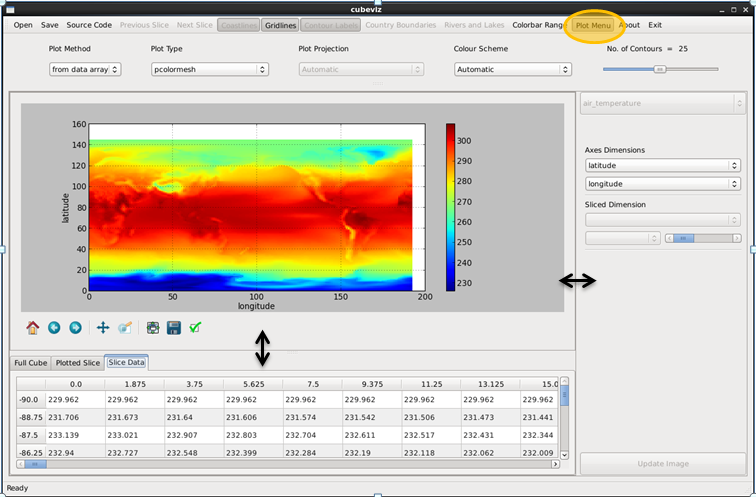
\includegraphics[width=90mm]{tute4.PNG}
\caption{Drag where the arrows are to change the layout of the window. Click on
Plot Menu to toggle the Plot Menu on and off.}
\label{overflow}
\end{figure}

Likewise, you are able to click as indicated here and drag left or right to
change the size of the cube options section.

Finally, the plot menu can be toggle on or off by clicking the 'Plot Menu'
button.

\subsubsection{Change the Plot Type}

Changing the plot type is simple. Just click on the drop down list labeled
Plot Type, and select the type of plot you would like.

\begin{figure}[H]
\centering
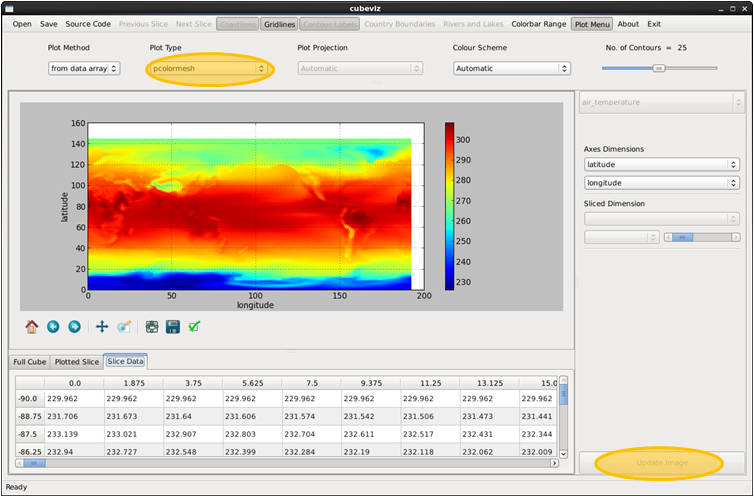
\includegraphics[width=90mm]{tute5.PNG}
\caption{Click here to change the plot type.}
\label{overflow}
\end{figure}

After having made any changes, you will need to click update (shortcut rtrn)
before the plot will be redrawn with the new options.

\subsubsection{Pick a Color Scheme}

Again, simply click on the marked drop down list and pick from the list.

The application currently uses the brewer color palletes that are compatible
with Iris.

\begin{figure}[H]
\centering
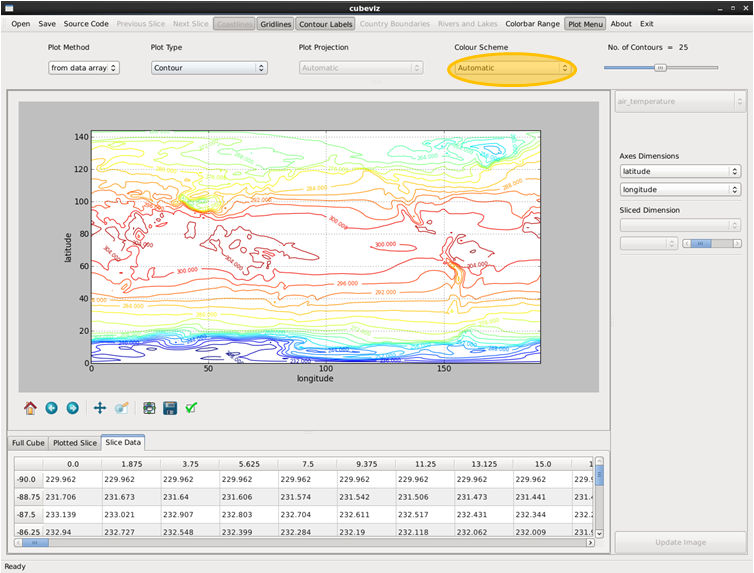
\includegraphics[width=90mm]{tute6.PNG}
\caption{Click here to change the colors used in the plot.}

\label{overflow}
\end{figure}

\subsubsection{Switching to quickplot}

So far, we have not been using any of the Iris plotting tools. Instead, we have
simply been plotting the raw data. This has the advantage of being very fast,
but comes without much of the functionality offered by Iris and Cartopy. Lets
switch now to using iris.quickplot for creating the images. This can be done
by clicking on the plot method button and selecting using quickplot from the
drop down list. Click update to replot the graph.

\begin{figure}[H]
\centering
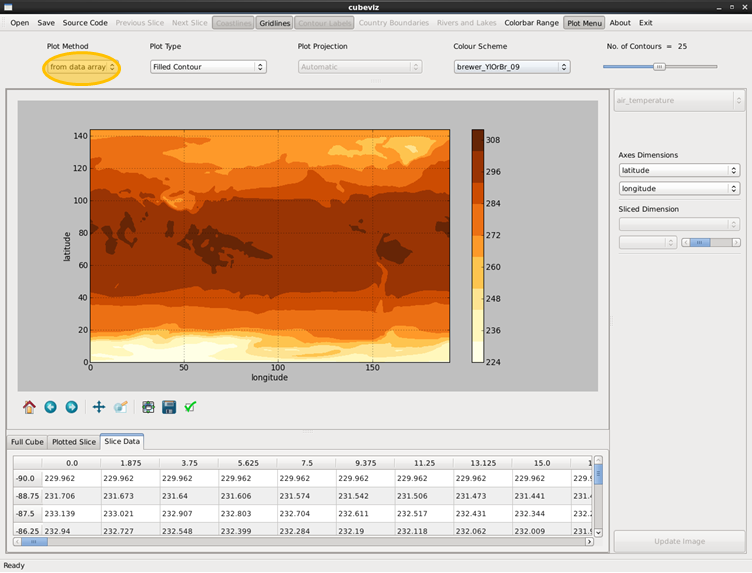
\includegraphics[width=90mm]{tute7.PNG}
\caption{Click here to change the plot method.}
\label{overflow}
\end{figure}

\subsubsection{Contours, Coastlines and More}

Now that we are using quickplot, you will notice that there are more options
enabled in the toolbar. The ones
availiable for this cube are coastlines, country boundaries, rivers and lakes
and contour labels if the plot type is Contour.

You also have the option to change the number of contours plotted using the
slider.

Try turning these options on and off now to get a feel for them.
(remeber that you will need to click update before the plot is redrawn)

\begin{figure}[H]
\centering
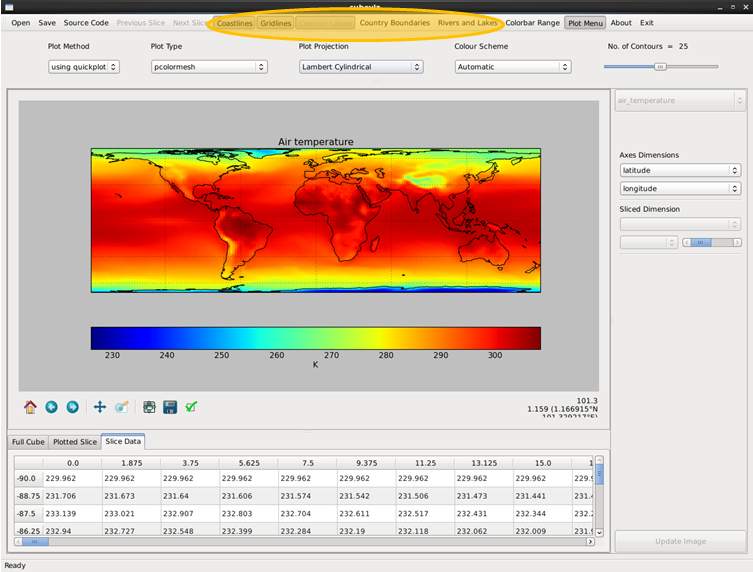
\includegraphics[width=90mm]{tute9.PNG}
\caption{This range of options will affect what is plotted on the image.}
\label{overflow}
\end{figure}


\subsubsection{Choose a Projection}

Just as simple to change. Click on the Select Projection box, and make a choice.

\begin{figure}[H]
\centering
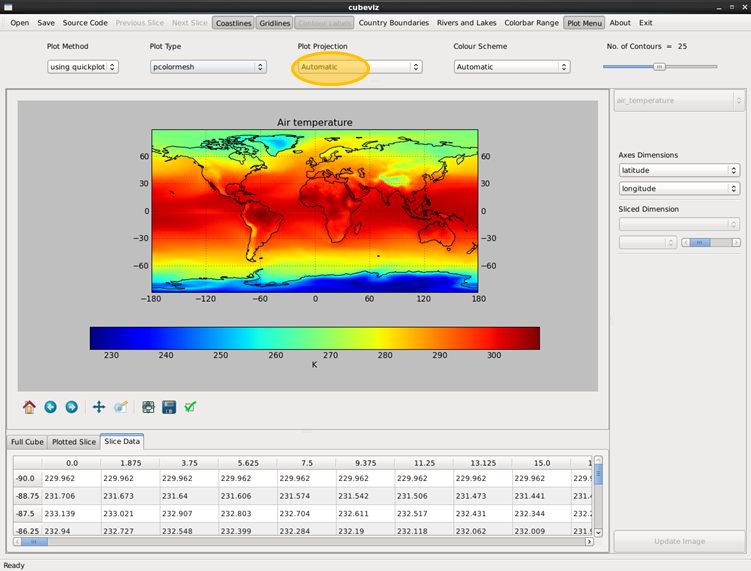
\includegraphics[width=90mm]{tute8.PNG}
\caption{Clicking here will change the progrection that is being used.}
\label{overflow}
\end{figure}

However, at the time of writing, some bugs in Cartopy make many of the
projections very tempremental. (This is known about and being fixed)

As such, a few of the projections have temporarily been removed from the
program. You may also see other bugs when using projections. It would be
greatly appreciated if you could report any bugs that you find.


\subsubsection{Matplotlib Interactions}

In just the same way as if you had plotted the graph through the terminal,
you have all of the same options with you matplotlib image. The standard
toolbar can be found below the image and provides functionality for
zooming, dragging etc.

\begin{figure}[h]
\centering
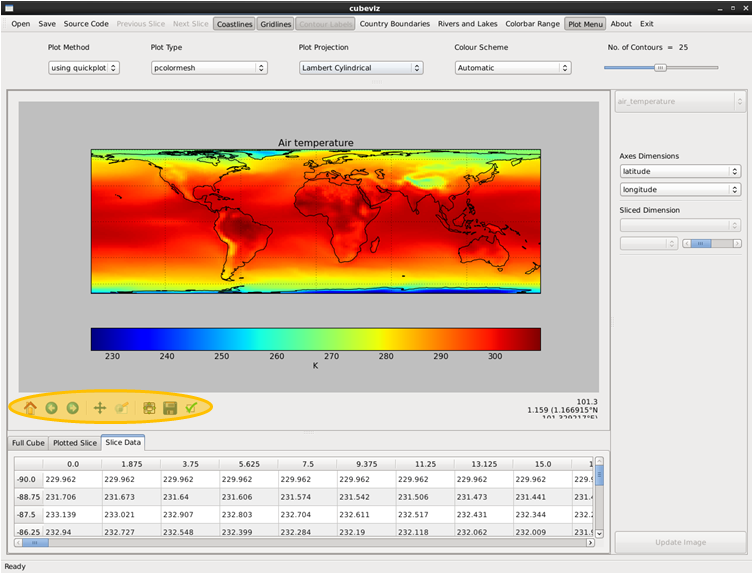
\includegraphics[width=90mm]{tute10.PNG}
\caption{These options are the same as those found in a standard matplotlib
toolbar.}
\label{overflow}
\end{figure}

\subsubsection{Saving your Image}

You can save your image either by clicking the save button on the matplotlib
toolbar, or by clicking save on the main toolbar. In both cases you will open a
file browser which will allow you to save the image as normal.

You can save the image in numerous formats including png and jpeg.

\subsection{More Complex Cubes}

In this next example, we are going to load a 4 dimensional cube. Following the
same method as before, this time load the 'A1B\_north\_america.nc' file.

\subsubsection{Arranging Dimensions}

If we now look at the cube information section, and flick between the tabs, we
can see that there is now a difference between the full cube and cube slice
summaries.

\begin{figure}[H]
\centering
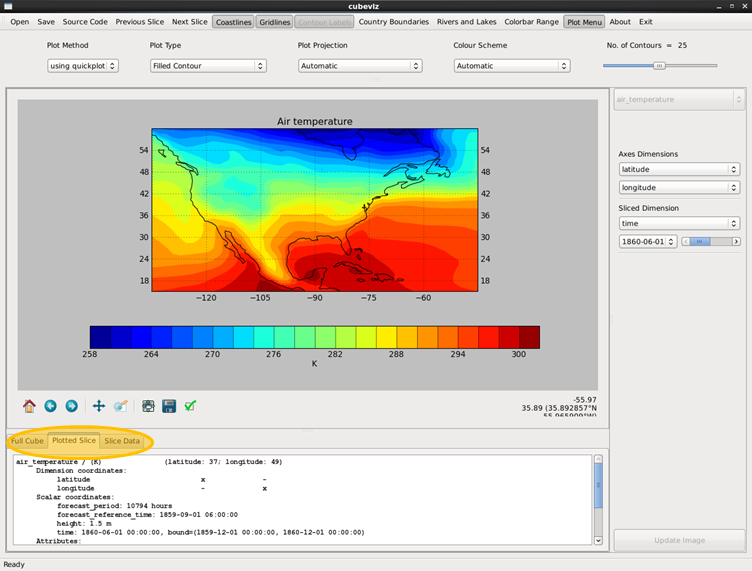
\includegraphics[width=90mm]{tute11.PNG}
\caption{Inspect the current slice using these buttons.}
\label{overflow}
\end{figure}


Looking closer at the Sliced Cube tab, we can see that the Axes Dimensions
correspond to the dimensions of this cube slice, and that the other two
dimensions have been collapsed down to the value shown on the boxes (although
if the coordinate is time then there may be differences as Iris transforms
the time values)

We can now try changing the Axes dimensions.

Click on the latitude axes dimension and change it to be time.
Now click update (or press rtrn) to plot the new graph.

\begin{figure}[H]
\centering
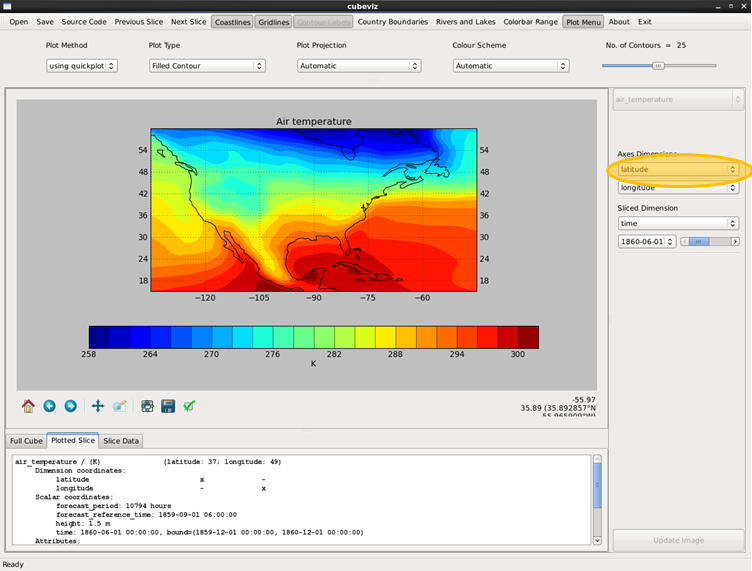
\includegraphics[width=90mm]{tute12.PNG}
\caption{Change the coordinate from latitude to time.}
\label{overflow}
\end{figure}


Notice that now many of the options have been removed. For example you now
cannot plot coastlines or change the projection. This is because the plot is
no longer a lat/lon plot, so these options would make no sense.

\subsubsection{Moving through a Dimension}

To move through the slices, you can either select the slice you would like to
see using the slider or the drop down list, or you can use the next and previous
slice buttons (shortcuts 6 and 4) to step through the slices.

\begin{figure}[H]
\centering
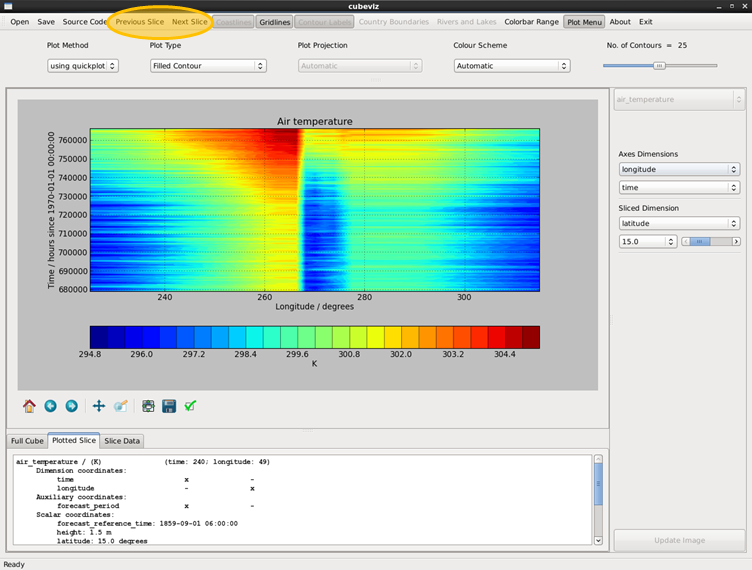
\includegraphics[width=90mm]{tute13.PNG}
\caption{Use these to move through the slices.}
\label{overflow}
\end{figure}

\subsubsection{Setting the Colorbar}

As you are moving through the slices, you may have noticed that for every new
slice, the colorbar updates. This makes it difficult to compare between the
slices, as red in one slice may not be the same temperature as red in any other
slice.

To change this, click on the Colorbar Range button.

\begin{figure}[H]
\centering
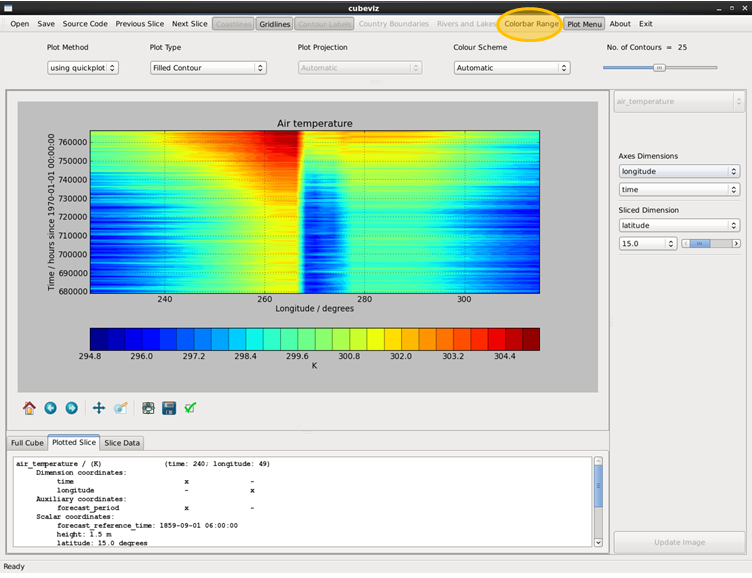
\includegraphics[width=70mm]{tute14.PNG}
\caption{Click here to open the colorbar dialog box.}
\label{overflow}
\end{figure}

This will open a new window. In this window, check the box next to Fix across
all Slices. You will notice that the values in the max and min boxes will change.

Closing this and again moving through the slices, you will notice that it is
now much easier to compare between slices, as a particular color will now
always correspond to the same temperature.

\begin{figure}[H]
\centering
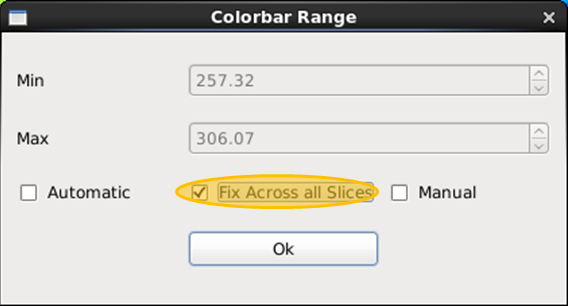
\includegraphics[width=90mm]{tute15.PNG}
\caption{Clicking here will fix the colorbar over all of the slices.}
\label{overflow}
\end{figure}

What we have done here is to scan through all of the slices, and set red to be
the maximum value across all of the slices, and blue to be the minimum across
all of the slices.

You are also able to specify your own range for the colorbar by clicking the
manual botton in the Colorbar Range window and then changing the max and min
values. Try this now a see what effect this has.

\subsection{More Dimensions}

For the last section al the tutorial, try opening a four dimensional cube. One
such cube is 'uk\_hires.pp', again found in the Iris Sample Data folder.

\subsubsection{Selecting a Cube from a File}

Looking at the Select Cube box, you will see that unlike in the last example,
this box is now enabled. Click it, and you will see that you now have a choice
of the 2 cubes contained within this file.
(remembering still that the update button must be pressed before the graph will
be redrawn)

\begin{figure}[H]
\centering
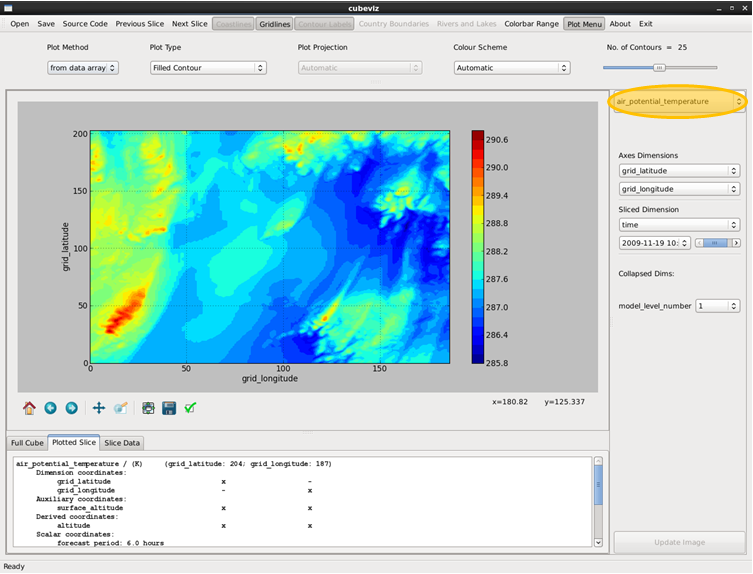
\includegraphics[width=90mm]{tute16.PNG}
\caption{Click here to change the current cube within the file.}
\label{overflow}
\end{figure}

\subsubsection{Working with Collapsed Dimensions}

Switch back to the air\_potential\_temperatur cube. You should now be able to
see that we have filled one of our collapsed dimension
slots. Checking the Cube Slice tab, you will see that the cube has been
collapsed down onto the value specified next to the collapsed dimension name.

To change this value, simply select a new one from the drop down list.

To change which dimenions are collapsed, just pick the dimensions that you
would like to plot as before.

\vspace{4mm}

That's it! You have now seen all of the features availiable to you, and
hopefully feel ready to start using Cubeviz.

If you have any further questions or have any problems, please contact $....$

\pagebreak

\section{Keyboard Shortcuts}

\begin{table}[h]
\caption{Keyboard Shortcuts}
\centering
\begin{tabular}{c c}
\hline\hline
Action & Shorcut \\ [0.5ex]
\hline
Open & Cntl + O \\
Save & Cntl + S \\
Update & rtrn \\
Previous Slice & 4 \\
Next Slice & 6 \\
Coastlines & C \\
Gridlines & G \\
Contour Labels & L \\
Country Boundaries & B \\
Rivers and Lakes & R \\
Colorbar Range & O \\
Plot Menu & M \\
Exit & Esc \\ [1ex]
\hline
\end{tabular}
\label{table:shortcuts}
\end{table}

\end{document}